\documentclass[crop]{CSLB}%%%%where CSL is the template name

%The authors can define any packages after the \documentclass{CSL} command.
\usepackage{amsmath} %for dealing with mathematics,
\usepackage{amsthm} %for dealing with theorem environments,
\usepackage{cite} %%%for dealing with citations
\usepackage{hyperref} %for linking the cross references
\usepackage{graphics} %for dealing with figures.
\usepackage{algorithmic} %for describing algorithms
\usepackage{subfig} %for getting the subfigures e.g., "Figure 1a and 1b" etc.
\usepackage{url} %It provides better support for handling and breaking URLs.

%\usepackage{natbib}
\usepackage{boites}

%\usepackage{graphicx}
%\usepackage{float}
%\usepackage{psfig}
%\usepackage{amsfonts,amssymb}
%\usepackage{color}
%\usepackage{textcomp}
%\usepackage[T1]{fontenc}
%\usepackage{aecompl}
%\usepackage{times}
%\usepackage{txfonts}
%\usepackage[english]{babel}
%\usepackage[utf8x]{inputenc}
%\usepackage{amsmath}
%\usepackage{caption}
%\usepackage{siunitx} 

\jname{Astrobiology}%

\newtheorem{theorem}{Theorem}
\newtheorem{condition}{Condition}

\begin{document}

\bibliographystyle{mn2e}

\supertitle{Research Paper}

\title[Probabilities of SETI contacts]{Probability of causal
contact between interstellar civilizations through MonteCarlo simulations}

\author[Lares \& Funes]{Lares M$^{1, 2}$, Funes J$^{1, 3}$}

\corres{\name{Lares M} \email{marcelo.lares@unc.edu.ar}}

\address{
   %
   \add{1}{CONICET, Argentina}
   
   \add{2}{Universidad Nacional de C\'ordoba, Observatorio
   Astron\'omico de C\'ordoba, Argentina}
   
   \add{3}{Universidad Cat\'olica de C\'ordoba, Argentina}
   %
}

\begin{abstract}
%
The abundance of intelligent civilizations in the galaxy is a
longstanding question, which is often conceptualized as the problem
of the lack of received communication of the Fermi paradox.
%
Most efforts on the estimation of a number of intelligent
civilizations are centered on the Drake equation, although 
its factors are affected by large uncertainties, and it lacks a
temporal nature.
%
Here we present numerical simulations of stochastic processes of
emergence of civilizations with communication capabilities, and
the causal contacts among them.
%
We analyze the rate of causal contacts as a function of the mean
number of civilizations and the mean lifetime span distribution.
%
Our results indicate that, given the large distances involved, in
the odds to obtain a contact in a few years of monitoring, assuming a
perfect detection rate, are very rare.                                 
%
\end{abstract}

\selfcitation{Lares M, Funes J (XXXX).  Estimating the probability of
causal contact between civilizations through MonteCarlo simulations,
International Journal of Astrobiology}

\keywords{SETI, Computer simulations, Statistics}

\JELclassification{XX; XX}
\MSCcodes{XX; XX}

\Abbreviations{CETI: Communicating Extraterrestrial Intelligence, DE:
Discrete Event, GHZ: Galactic Habitable Zone}

\maketitle

\Fpagebreak





\section{Motivations}
%\section{Motivations: Uncertainties and the non detection problem for ETI contact}
%{{{

A common approach to discuss the possible number of extraterrestrial
intelligent civilizations (ETI) has been the use of the Drake equation
\citep{Gleiser2010, Prantzos2013, Haqq-Misra2017}.
%
However, the uncertainties in the factors make it less prone to a
formal application to define searching strategies or to compute
actual numbers, but is used to organize the discussion instead.
%
Some modifications to the original idea of the equation have tried to
imprint a stochastic nature, or to propose a probabilistic approach,
or to consider the temporal structure which is missing in the
equation.
%
Temporal aspects of the distribution of communicating civilizations
and their contacts have also been explored by several authors
\citep{Fogg1987, Forgan2011, Balbi2018},
%The Impact of the Temporal Distribution of Communicating Civilizations on Their Detectability
%Temporal dispersion of the emergence of intelligence: an inter-arrival time analysis
%The spatiotemporal aspects of SETI
%
as well as efforts on considering the stochastic nature of the Drake equation
\citep{Glade2011}.
%
The simulation approach has also benn considered
\citep{Forgan2008, Forgan2010}.
%New numerical determination of habitability in the Galaxy: the SETI connection
%
Since the factors in the Drake equation are uncertain, we propose to
avoid the frequentist approach of this equation
and to explore a parameter space, where instead of computing a final
number, we provide a statistical distribution that gives conditional
probabilities.
%
The only fact that can be stated with certainty is that for the number
of years SETI projects have been working we have not received any
signal within the conditions stablished by SETI.



The discrete events method for simulating a stochastic process is an
approximation that allows to study the behaviour of complex
systems, by considering a sequence of well defined discrete events.
%
The simulation os carried out by following all the variables that
describe the system, that constitute the state of the system.
%
The evolution of the process, then, is described as a set of changes
in the state of the system.
%
In this context, an event produces a specific change in the state,
that can be triggered by random variables that encode the stochastic
nature of the physical phenomenon.
%
The process involves following the changes on the state of the system,
definig the initial and final states, defining a method that allows to
keep track of time progress, and maintaining a list of relevant
events.


In a recent work, \citep{Balbi2018} use a statistical model to analyze
the occurrence of causal contacts between civilizations in the Galaxy.
%
The author highlights the effect of evolutionary processes when
attempting to estimate the number of communicating civilizations that
might be in causal contact with an observer located on the Earth.



\citet{cirkovic_temporal_2004} also emphasize the lack of temporal
structure in the Drake equation.



%While the Drake equation remains a very useful
%guide in identifying and analyzing the various factors in-
%volved in the problem and their relative probabilities, our
%approach could provide a better framework with which to
%perform a statistical analysis when taking into account evo-
%lutionary processes. In particular, we have shown that the
%Drake equation can misestimate the number of detectable
%communicating species if spatial and temporal dependencies
%are important. This should suggest some caution in the un-
%critical application of such an equation. In this paper, we offer
%an exemplificative illustration of the effect of different
%probability distributions for the typical timescales involved
%in the problem. Ideally, it would be desirable to arrive at a
%mathematical description of such distributions based on a
%modeling of the underlying astrophysical and biological
%processes. This points out a possible future direction of in-
%vestigation in which an integrated evolutionary (and coevo-
%lutionary) approach to the problem would be a central focus
%of interest (for more on this perspective, see, e.g., Chaisson



In this work we address the problem of the temporal and spatial
structure of the distribution of communicating civilizations, by
exploring the hypothesis space over a minimal set of parameters.
%
In Sec.~\ref{S_methods} we introduce the methods and discuss the candidate
distributions for the statistical aspects of the times involved in the
communication process.
%
Then, we present our results in Sec~\ref{S_results}, with special emphasis on
the statistical distributions of the duration of causal contacts in one or
both directions, the possible differences on the position of a
civilization on the Galaxy and the distribution of time intervals for
the waiting of the first contact, always as a function of the three
simulation parameters.
%
Finally, in Sec.~\ref{S_discussion} we discuss our results and future research
directions.


%}}}



\section{Methods and working hypotheses}

%: accounting for causal contacts with 
%discrete event simulation process}\label{S_methods}
%{{{

Some complex stochastic processes can be efficiently modeled with the
discrete--event (DE) simulation approach.
%
Simulations are suitable tools to analyze systems that evolve with
time and involve randomness.
%
In general, simulations require less assumptions and simplifications
than theoretical approaches, and can be applied to systems where a
theoretical model can not be found.
%
A system described with the DE paradigm is characterized by a set of
actors and events, where actors interact causally through a series of
events on a time line and process these events in chronological order
\citep{ptolemaeus_system_2014, chung_simulation_2003,
simulation_ross_2012}.
%
This method is well suited for the 
particular case of the difusion of intelligence signals in
the Galaxy.
%
Assuming some simple hypotheses, 
the discrete events method can be performed taking into
account a small number of variables, which allows to analyze the
results as a function of those variables.


In what follows, we describe the experimental setup chosen to estimate
the probabilities of causal contacts and several derived quantities in
terms of three independent parameters, namely, the mean time span
between the appeareance of consecutive communicating civilizations
($\tau_a$), their mean lifetime ($\tau_s$), and the maximum distance a
signal can be detected by another civilization ($D_{max}$).
%
Intuitively, the shorter $\tau_a$ and the larger $\tau_s$ and
$D_{max}$, there is a greater probability of the existence of causal
contacts between pairs of intelligent civilizations in the Galaxy
(Table \ref{T_simu}).
%
The causal connection can be produced without the need of the two
civilizations being concurrent or active at the same time.
%
Each CETI will fill an annular region of the Galaxy, limited by two
surfaces.
%
The leading front, or surface of first contact (SFC) grows from the
central CETI until it reaches the distance $D_{max}$.
%
The trailing front, or surface of last contact (SLC) also grows from
the central CETI, with a delay with respect to the SFC equivalent to
the lifetime of the CETI, and produces an annular region that shrinks
until it reaches $D_{max}$, when all signal from the central CETI is
lost.
%
In the 2D simulation only the intersection of these spheres with the
plane of the galaxy is relevant, and produce the corresponding
circumferences.





The temporal structure of the process is defined by two distribution parameters that
represent the mean time interval that an intelligent civilization can
emit and receive signals, and the mean time interval between the
emergence of an intelligent comunicating civilization and the next
one.
%
The spatial structure of the simulation is given by the size and shape
of the Galactic Habitable Zone and the maximum distance a signal can
travel to be detected.
%
The parameters for the temporal distributions also determine the
spatial properties since the density of active cetis in the Galaxy depend on these
two parameters.
%
For example, a small $\tau_a$ and a large $\tau_s$ will produce a
Galaxy densely populated woth CETIs, and viceversa.
%
Also, some hypotheses must be made in order to complete the
simulation.
%
Firstly, we assume that the distribution of the appeareance of new
CETIs is a stationary Poisson distribution.
%
Regarding the duration of a CETI, we propose that the distribution of
the duration of CETIs is a stationary exponential distribution.
%
\citet{Balbi2018} stress the fact that it would be desirable to arrive
at a theoretical statistical distribution of the lifespan of
civilizations, preferentially on the basis of the underlying
astrophysical and biological processes.
%
\citet{Maccone} argues that this distribution should be a log normal.
(EXPAND)




There is no a temporal window for the model, i.e., the simulation
starts when the process is already stable, and ends before any
galactic effect could modify or affect of fixed variables.
%
The probability for the rise of a CETI is homogeneous over the GHZ.
%
Although the Galaxy has a well known spiral structure, the assumed
sparcity of civilizations makes this assumption very reasonably.
%
Otherwise, if the distribution of civilizations is not sparce, it
could be the case that the spiral arms would host most of the
civilizations, and contacts are frecuent between closely located
civilizations.
%
In such a case we could expect that the interpretation of our results
could be considered as pesimist for the stablishment of a contact with
our planet.
%
We also limit the posibilities of life or other types of civilizations
to the hypothesis usually stated for the definition of the GHZ.
%
This means that we set aside possibel civilizations that could survive
in severe conditions or unstable systems, which would prevent the
appeareance of life as we know it.

 
\setlength{\tabcolsep}{10pt}
\begin{table}
\centering
\begin{tabular}{cl}
\hline
   \multicolumn{2}{l}{independent variables} \\
\hline
   $\tau_{a}$ & Mean temporal separation between\\
              & consecutive awakenings \\
   $\tau_{s}$ & Mean lifetime of a CETI \\
   D$_{max}$ & Maximum reach of a message \\
\hline
\multicolumn{2}{l}{fixed variables and assumptions} \\
\hline
   & All CETIs share the same statistical properties\\
   & The process is homogeneous \\
   & The scan of the sly is fully efficient\\
   & Absence of panspermia or colonization \\
   & The GHZ is a 2--dimensional ring \\
20000ly    & Inner radius of the GHZ \\
60000ly    & Outer radius of the GHZ \\
1.e6 y    & Time span of the simulation \\

\hline
\end{tabular}
\caption{Definition of independent variables and fixed paramenters 
   that are part of the simulation.}
\label{T_simu}
\end{table}
 

While the aforementioned assumptions are basic conditions for most of
the stochastic processes observed in nature, 
we need to make stronger assumptions related to the nature of the
message.
%
The most simple assumption about the message itself, is that it
travels at light speed.
%
With this, we are considering messages sent through, for example,
electromagnetic radiation or even gravitational radiation, but we set
appart messages sent with mechanical means or physical objects, or
through some unknown technology that violates the known so far laws of
physics.
% 
For the communication of CETIs through messages sent isotropically, 
we assume that the capacity to emit signals and to receive
signals ocurr at the same time.
%
This means that the ability to find another civilization develops at
the same time that the ability and intention to emit a signal in all
direction, intented to be detected by an unknown civilization.
%
Although there are several reasons to think that this could not be the
case, at large time scales it can be considered that both abilities
occurr roughly at coincident epochs.
%
Another essential assumption is that all CETIs use the same signal power, so that there is a maximum distance out to which it can be detected.
%
It is worth mentioning that we are considering in our experimental
setup a system composed by several emmiters and receivers across the
Galaxy, under the hypothesis proposed before.
%
In such a system we compute probabilities of a CETI making contact
with another CETI, and the results must be interpreted as for a
randomly chosen CETI, given certain conditions of homogeneityon an
ensemble of equivalent galaxies.
%
We stress the fact that we are not centered on the probabilities for
the Earth itselft, but on a generalized CETI.
%
Regarding the extent of the signals, we know that the distance from
which a signal from Earth could be detected using the current
technology is of a few hundreds light years, given that the signal was
sent to a specific direction.

%https://setiathome.berkeley.edu/forum_thread.php?id=80585&postid=1833000#1833000]
%https://www.engadget.com/2017/05/25/listening-to-starlight-our-ongoing-search-for-alien-intelligenc/]
%[from https://en.wikipedia.org/wiki/Fermi_paradox]
%
It is straightforward to propose and implement a distribution of
maximum distances, although this would increase the model complexity
at the cost of a larger uncertainty or of another dimension on the
hypothesis space.
%
This proposal is based on a pronoid scenario (REF), and we do not
consider in this work the ocurrence of paranoid or partially paranoid
civilizations.
%
If that would be the case, the results obtained here can be taken as
upper limits.



In our simulations we also assume the simplest situations for the
growth of ETIs.
%
For example, we discard the possibility of stellar colonization
(Walters 1980) and assume that the communication aim is performed to
all directions with the same power and the same probability, i.e.,
strongly assume isotropic communication in all cases.
%
More detailed simulations could be produced considering different 
efficiency of communication or detection methods.
%
Also, a mixed paranoid/pronoid population of intelligent civilizations
could be implemented easily.
%
However, in this case we also would complicate the experimental setup,
make the results less evident.
%
The results are independent of the nature of life (organic or
artificial).
%
The lifetime of a civilization can be caused by autodestruction or by
external factors.




\subsection{Power laws vs. exponential laws}

The exponential distribution of lifespan and waiting times is
justified by considering that the process of appeareance of life in
the galaxy is homogeneous and stationary.
%
This means that there is no preferred location within the GHZ for the
spontaneos appeareance of life, and that the emergence of a
civilization is independent of the existence of previous civilizations 
in the galaxy.
%            
This is equivalent to proposing a Poisson process for the emergence of
CETIs, since there is a close relation between the number of events in
time or space and the waiting time or separation, respectively.
%
That is, these are two alternative approaches to describing the same
process, a Poisson distribution for the number of events implies an
exponential distribution for their sepations, and viceversa.
%
It should be emphasized that the exponential laws used in this work
are assumed, although instead of analyzing results from a particular
parameter chosen ad--hoc, we explore the hypothesis space and analyze
the impact of the values of these parameters on the results.
%                                                           

The power law and exponential statistical distributions are among the
most common patterns found in natural phenomena.
%
For example, the distribution of the frecuency of words in many
languajes is known to follow a Zipf law (which is a power law).
%
Zipf law also describes population ranks of cities in various
countries, corporation sizes, income rankings, ranks of number of
people watching the same TV channel (Zipf's law entry on Wikipedia).
%
The magnitudes of earthquakes, hurricanes, volcanic eruptions and
floods; the sizes of meteorites or the losses caused by business
interruptions from accidents, are also well described by power laws
(Sornette 2006).
%
The power law behaviour has been observed in a variety of systems,
including for example stock market fluctuations, sizes of computer
files and word frequency in languages \citep{mitzenmacher_brief_2004,
Newman_power_2005, simkin_theory_2006}
%
Power laws have also been widely used in biological sciences, e.g., in
analysing connectivity patterns in metabolic networks
\citep{jeong_large_2000} and in the number of species observed per
unit area in ecology \citep{garcia_origin_2006, frank_common_2009}.


\subsection{Discrete event process}

Given a set of parameters $(\tau_a, \tau_s, D_{max})$, the functional
forms of the statistical distributions and fixed values
for the hypotheses, a discrete
event simulation is performed by keeping track of a set of variables
that change each time a meaningful event is produced.



\setlength{\tabcolsep}{10pt}
\begin{table}
\centering
\begin{tabular}{cccc}
\hline
   fixed parameter & \multicolumn{3}{c}{adopted value}\hfill \\
\hline
   inner GHZ radius\hfill & \multicolumn{3}{c}{20000 ly}\\
   outer GHZ radius & \multicolumn{3}{c}{60000 ly}\\ \\
\hline
   variable parameter & min & max & N \\
\hline
   D$_{max}$ & 1000 ly & 20000 ly & 20\\
   $\tau_{a}$ & 1000 y & 20000 y & 20\\
   $\tau_{s}$ & 1000 y & 20000 y & 20\\
\hline
\end{tabular}
\caption{Adopted values for simulation parameters. Fixed parameters
   define the GHZ.  Variable parameters define the temporal structure
   of the process and the reach of messages.}
\label{T_parameters}
\end{table}



The main variables that follow the evolution of the simulation are:

\begin{itemize}
   \item Position of stars.  Sampled randomly within the GHZ
   \item Time of the awakening of each CETI
   \item Time of the vanishing of each CETI
\end{itemize}

The variables that can be deduced from the previous ones are:

\begin{itemize}
   \item Number of CETIs in casual contact with at least another CETI
      at a given time.
   \item Number of CETIs as a function of time
   \item Number of CETIs that receive a message at least one time
   \item Number of CETIs that receive a message at least one time and
      successfully deliver an answer.
   \item Number distribution of waiting time to receive a message
\end{itemize}




\subsection{Exploration of the hypothesis space}






%========================================================================
%========================================================================
%========================================================================
                   

\begin{figure}
   \centering
   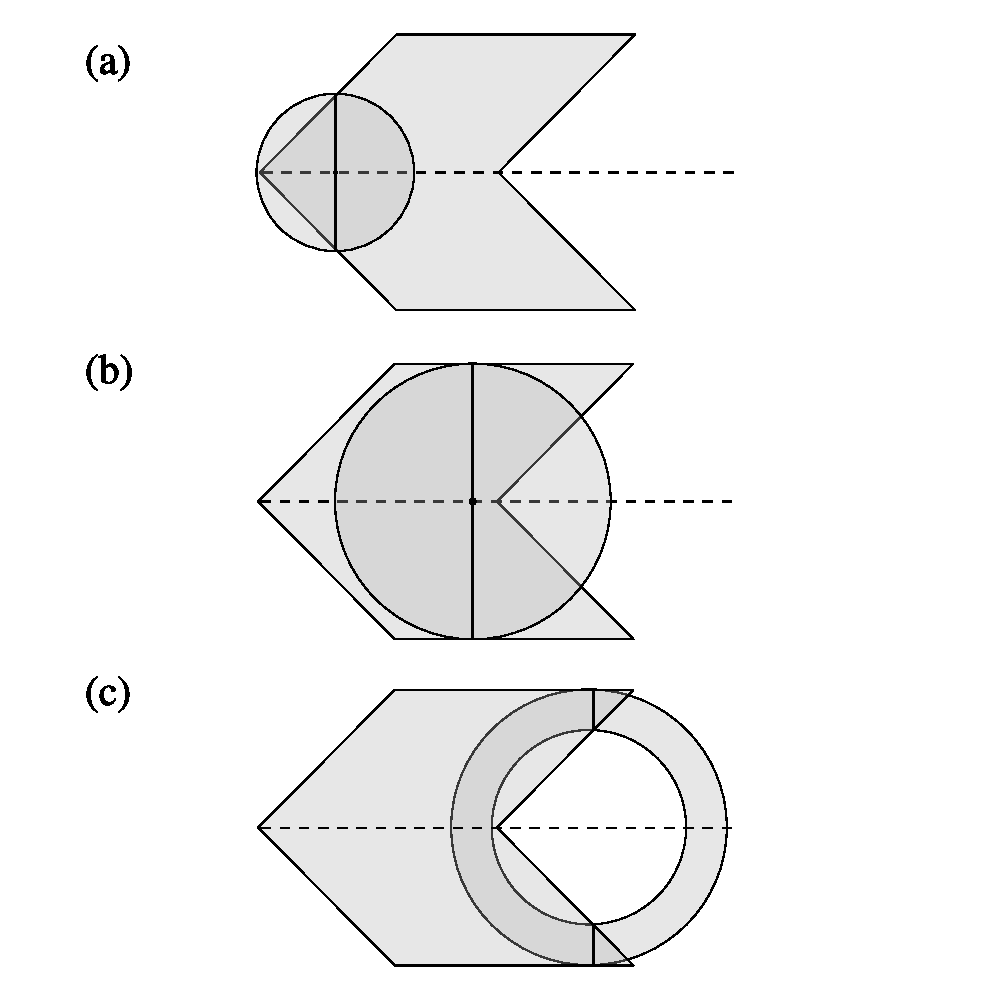
\includegraphics[width=0.5\textwidth]{growingsphere.pdf}
   \caption{Schematic representation of the growing communicating
   sphere, over the space--time diagrams, where time is represented on
   the horizontal direction, and space is represented in the vertical
   direction.  In (a) the sphere is
   growing as the surface of first contact has not reached the maximum
   distance.  In (b) it has reached the maximum distance, so that it
   remains at the same size.  After a Doomsday event, the signals can
   still be observed, but the surface of last contact grows }
   \label{F_sphere}
\end{figure}

  
\begin{figure}
   \centering
   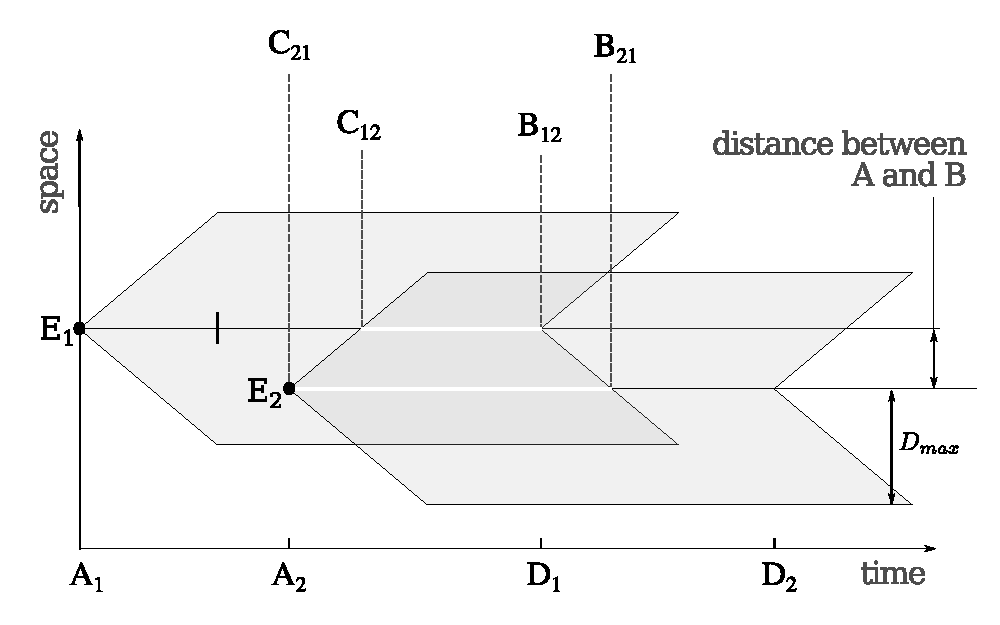
\includegraphics[width=0.5\textwidth]{abcd.pdf}
   \caption{Schematic representation of two emitters, $E_1$ and $E_2$,
   that reach each other at different times.  The time span for $E_i$
   is $(A_i, D_i)$, for $i=\{1,2\}$.  Emitter $i$ can listen to
   emitter $j$ between $C_{ij}$ and $B_{ij}$.
   The type and length of causal contact in both directions depend on
   the distance and time lag between the awakening events, the maximum
   distance that a signal can reach and the time period in which each
   emitter is active.}
   \label{F_abcd}
\end{figure}
                     

Possible hypothesis improvements are:

\begin{itemize}
   \item Dmax is different for different CETIs.  For example a power
      law where powerfull emmisions are rare and weak emssions are
      common.
   \item The probability of the rising of a new CETI vary within the
      GHZ.
   \item Correction by coverage ratio in the detection and by
      targetting ratio in the emission.
   \item Spiritual factor.  Explore the role of the S factor: message
      contents, influence on the lifespan of a CETI that receives a
      message, mean lifespan of a CETI that emits a message.
\end{itemize}


\subsection{Model for CETIs}


Since the method is based on events, the first step is to define an
architecture of events, the relationships between them and how events
trigger changes on the state of the system.
%
We consider a simulated system that represents the galactic habitable
zone (GHZ).
%
On a first approach, the GHZ is a 2-dimensional annular region.
%
The adopted values for the GHZ are XX and XX \citep{Lineweaver2004}.
%
This simple model does not take into accont the variations in stellar
density given by the spiral structure.
%
Although there are several possible approaches, we chose to follow the
evolution of the system according to the following events:

\begin{enumerate}
   \item[(A)] A new CETI appears (Awakening)
   \item[(D)] An old CETI dissappears (Doomsday)
   \item[(C)] A new causal contact is stablished (Contact)
   \item[(B)] An existing causal contact is interrupted (Blackout)
\end{enumerate}

The event of type B is produced when one of the two CETIs halts in its
capability of emmiting and receiving signals.



%======================================================================
%======================================================================
%======================================================================


The system is updated each time an event is produced.
%
The time marks for each event (A and D for each CETI and C and B for
each causal contact) are stored as a result of the simulation.
%
Also, the list of active CETIs is obtained as a function of time.
%
Some fixed variables must be set in order to carry out the simulation,
namely:

\begin{itemize}
   \item Size of the Galactic Habitable Zone,
   \item mean lifetime of a CETI, $\lambda_1$,
   \item mean waiting time for the appeareance of another CETI,
      $\lambda_2$, and
   \item maximum distance a message can be detected.
\end{itemize}

The Galactic Habitable Zone is the only one of the four parameters
that is barely known, is set at fixed values of the inner and
outer radii, radial symetry is assumed, and the with of the
galactic disk is neglected compared to the radial size.
%
The two radii are measured in light years, with the aim to maintain a
single and comprehensive unit for both space and time coordinates. 



The simulation was implemented on a python code, which is publically
available\footnote{https://github.com/mlares/simu\_contact}




%Variables en el programa
%\begin{itemize}
%   \item Nact: Número de CETIs activas
%   \item Nsee: Número de contactos por cada CETI
%   \item Nccc: CETIs en contacto causal. Notar que una CETI puede tener múltiples
%contactos de otras CETIs. Para cada una de ellas, guardar:
%   \item ID: ID de la CETI emisora
%   \item ID: ID de la CETI receptora
%   \item t\_hola: tiempo del primer contacto
%   \item t\_chau: tiempo del último contacto
%\end{itemize}
%
%
%Caso 1: aparece una nueva CETI
%Modificaciones al estado del sistema:
%\begin{itemize}
%   \item Agregar la CETI “A” a la lista de CETIs activas
%   \item Sortear la duración de la actividad de comunicación de la CETI “A”
%   \item Sortear el intervalo de tiempo hasta la aparición de la próxima CETI:
%t\_WakeUp\_next
%   \item Agregar la CETI “A” al árbol
%   \item Identificar todas las CETIs que están a menos de D max de la nueva CETI, y
%actualizar la lista de tiempos
%\end{itemize}
%
%Caso 2: desaparece una CETI
%Modificaciones al estado del sistema:
%\begin{itemize}
%   \item Eliminar la CETI a la lista de CETIs activas
%\end{itemize}
%
%
%Caso 3: una nueva CETI entra en contacto causal
%Modificaciones al estado del sistema:
%\begin{itemize}
%   \item Agregar la CETI B a la lista de contactos de la CETI A
%\end{itemize}
%


%}}}
 
\begin{figure*}
   \centering
   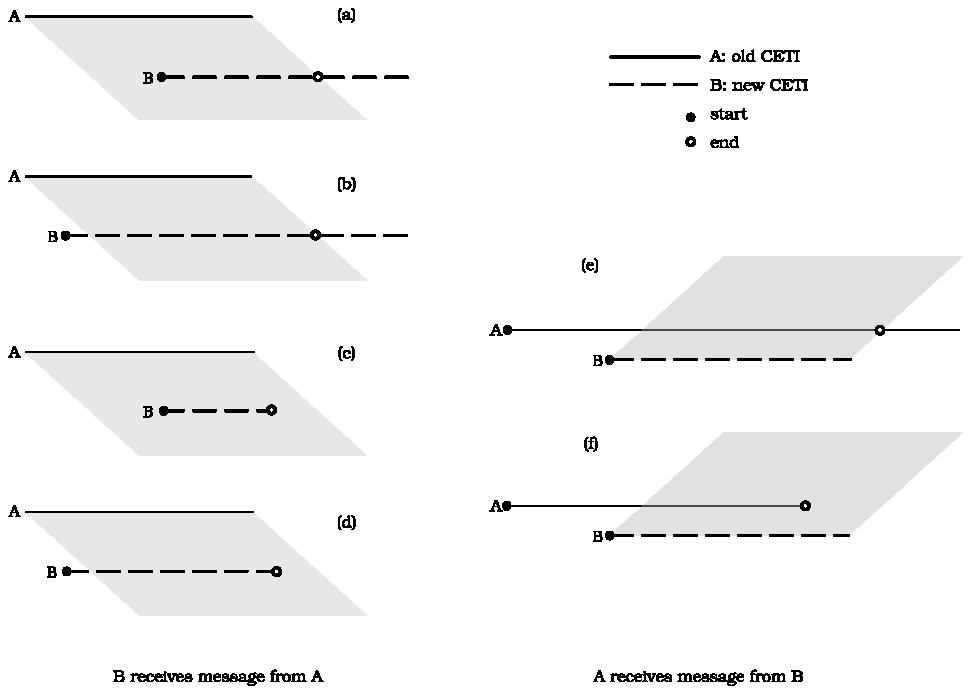
\includegraphics[width=\textwidth]{Messages_01.pdf}
   \caption{Schematic representation of the possible cases in which a
   ceti A can be in causal contact with a ceti B which appears later.
   The duration of the causal contact in one direction depends on
   several factors, mainly $\Delta t_A$, $\Delta t_C$, and $\Delta X$.}
   \label{F_messages}
\end{figure*}


 


\section{Results: exploring the parameter space}\label{S_results}
%{{{


We implemented the simulation of a regular grid of models varying over the
hypothesis space, which covers XXX different models.
%
For each model, we simulated XXX realizations with different random
seeds, in order to estimate the variance.
%
The simulated parameters, $\lambda_1$, $\lambda_2$ and $D_{max}$ cover
the range XX-XX, XX-XX and XX-XX, respectively, with a partition of XX
values for each parameter.





As a product of the simulations, several quantities are obtained.
%
Some quantities are directly derived from the discrete events, namely,
the ID of emitting CETI, the ID of emitting (receiving) CETI, the
position in the galaxy, the time of Awakening (Contact) and the time
of Doomsday  (Blackout) for each CETI.
%
This structure is always for the A-D cycle of each emitting CETI, and
repeats for each contact (C-B).
%
We can also derive the additional quantities.
%
The age of a CETI is the time elapsed from A to D.
%
%
%given time, ceti\_e is the CETI emitting signals (emiter), ceti\_r is
%the CETI receiving signals (receiver), ceti\_c is the ceti that
%listen at least another ceti (citizen) and ceti\_h is the CETI ceti
%that is lestened by at least another CETI.
%
The time span of a CETI listening another or being listened by another
can also be easily derived from the results of a realization.
%
This way we can also compute the distribution in the galaxy of cetis
that reach contact and the waiting time until the first contact or the
waiting time until the next contact.
%
Regarding the properties of the population of CETIs and its evolution,
we analyze the fraction of awaken time a ceti is listening at least
another ceti, the age of contacted CETIs at first contact, the
distribution of time to wait until next contact, the fraction of cetis
where the first contact is given at the awakening, the distribution of
the number of contacts for each CETI, the distribution of the maximum
number of contacts for each CETI, the distribution of the number of
contacts as a function of CETI age, the number of contacts as a
function of time in the galaxy, the rate of CETIs that succeed in
contact, and the distribution of distances between contacted CETIs.
%
Usefull derived quantity is the duration of two-way communication
channels the or the fraction of contacts that admit a response.
% 
We also analyze the relations between the distance to ceti vs. time of
double communication, the distance to ceti vs. age of contacted ceti,
the age of a ceti and the maximum number of contacted cetis before D,
or the lifespan of a ceti vs. max number of contacts.
%
All these quantities can be analyzed as a function of the simulation
parameters.
%



We chose eight models that are on fairly oposed regions of the
explored parameter space, and cover short/long lifetimes, short/long
waiting times for the next CETI to appear in the Galaxy and
short/large range reach of the signal, including all possible
combinations.
%
The details of each model are summarized in the
Table~\ref{T_SelectedModels}.


In Fig.~\ref{F_res_1} we show the Empirical cumulative distributions
of the number contacts for CETIs in four different samplas (M5, M6,
M7, M8) with long range signal reach (D$_{max}$=10000). 
%
The lifetime is more determinant than the awakening rate in increasing
the number of contacts.
%
As expected, of the four samples, the sample M7, which corresponds to
a dense awakening in the timeline and a long lifetime, is the model
that maximizes the number of contacts, reaching a maximum of order 100
contacts for a single CETI.
%
This is considerable larger than any model with a shorter lifetime,
which produce a number of contacts of at most the order of ten
contacts per CETI.
%
A couple of comments are worth to mention about this plot.
%
First, it has a logarithmic scale on the x-axis, and second it is the
cumulative, not differential, empirical distribution.
 



In what follows, we focus on the analysis of the duration of contacts
(Sec. X), the waiting time for the first contact (Sec. X) the
variations of contact posibilities as a function of the position of
the CETI in the Galaxy (Sec. X) and the occurrence of reciprocal
communication (Sec. X).
 



%}}}


\subsection{Duration of contacts}
%{{{

The duration of each contact for a single receiving CETI is given by the
time difference between a C event and a B event, which are direct
outputs for each simulation experiment.




%}}}


\subsection{Waiting time for a first contact}
%{{{

In this section we analyze the distribution of the waiting times for
a first contact.
%
Such distribution can be considered to compute the probability of
reaching a first contact within the first XX years.


In the Fig.~\ref{F_waiting} we show the fraction of the CETIs that
have made at least one contact  as a funtion of the elapsed time since
the awakening, given that they make at least one contact on their
lifetime.
%
From a frequentist approach, the normalizaed cumulative counts are
related to the estimation of the probability of observing a given time
with no success.
%             
XX panels show the histograms of the waiting times for the first
contact, for all the CETIs that make at least one contact along their
lifetime.
%
We show separately the histograms for several values of $\tau_a$ and a
fixed value of $(\tau_s, D_{max})$, and for several values of $\tau_s$ and a
fixed value of $(\tau_a, D_{max})$.
%
For different values of $\tau_a$, the shape of the distribution is
similar, so that a normalization ... but not in the case of different values of $\tau_s$.


%}}}



\subsection{Location within the Galaxy}
%{{{

%}}}



 
\setlength{\tabcolsep}{10pt}
\begin{table*}
\centering
\begin{tabular}{ccccc}
\hline
Model subset & D$_{max}$ & $\tau_a$ & $\tau_s$ & description  \\
\hline
M1 & 40000 & [10000, 30000]   & [10000, 50000]   &dense, short lifetime\\
M2 & 40000 & [170000, 190000] & [10000, 50000]   &sparse, short lifetime\\
M3 & 40000 & [10000, 30000]   & [400000, 440000] &dense, long lifetime \\
M4 & 40000 & [170000, 190000] & [400000, 440000] &sparse, long lifetime\\

M5 & 80000 & [10000, 30000]   & [10000, 50000]   &dense, short lifetime\\
M6 & 80000 & [170000, 190000] & [10000, 50000]   &sparse, short lifetime\\
M7 & 80000 & [10000, 30000]   & [400000, 440000] &dense, long lifetime \\
M8 & 80000 & [170000, 190000] & [400000, 440000] &sparse, long lifetime\\

\hline
\end{tabular}
\caption{Selected models to analize the behevior of some variables.}
\label{T_SelectedModels}
\end{table*}



  
\begin{figure} \centering
   %
   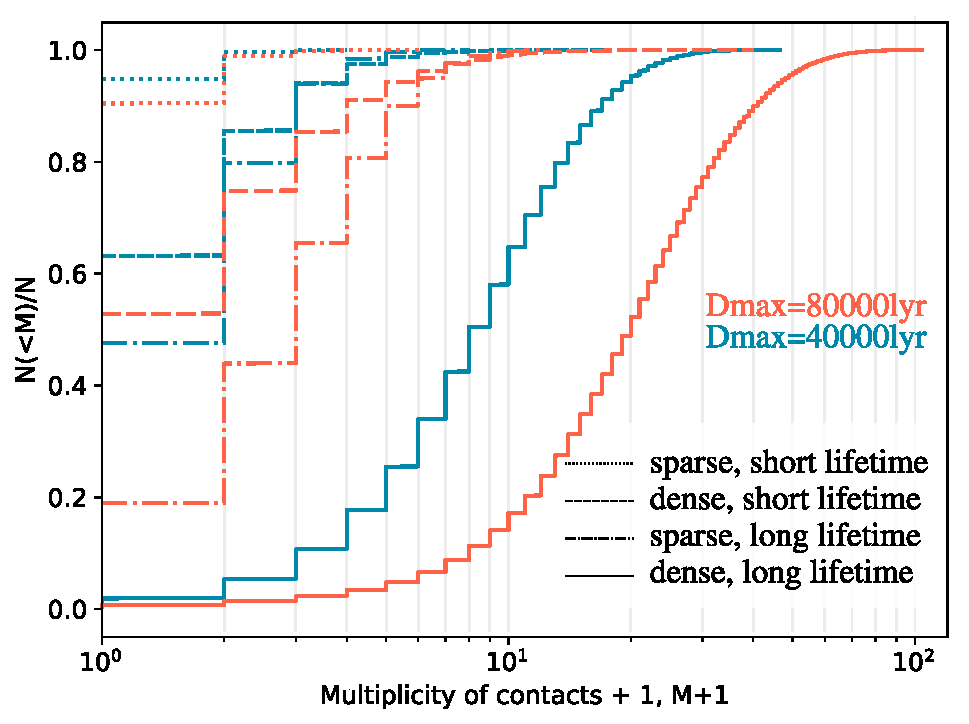
\includegraphics[width=0.5\textwidth]{F1.pdf}
   %
   \caption{Empirical cumulative distributions of the number contacts
   for CETIs in four different samplas (M5, M6, M7, M8) with long
   range signal reach (D$_{max}$=10000).
   %
   }
   % 
\label{F_res_1} \end{figure}
   
\begin{figure} % Distribution
   \centering
   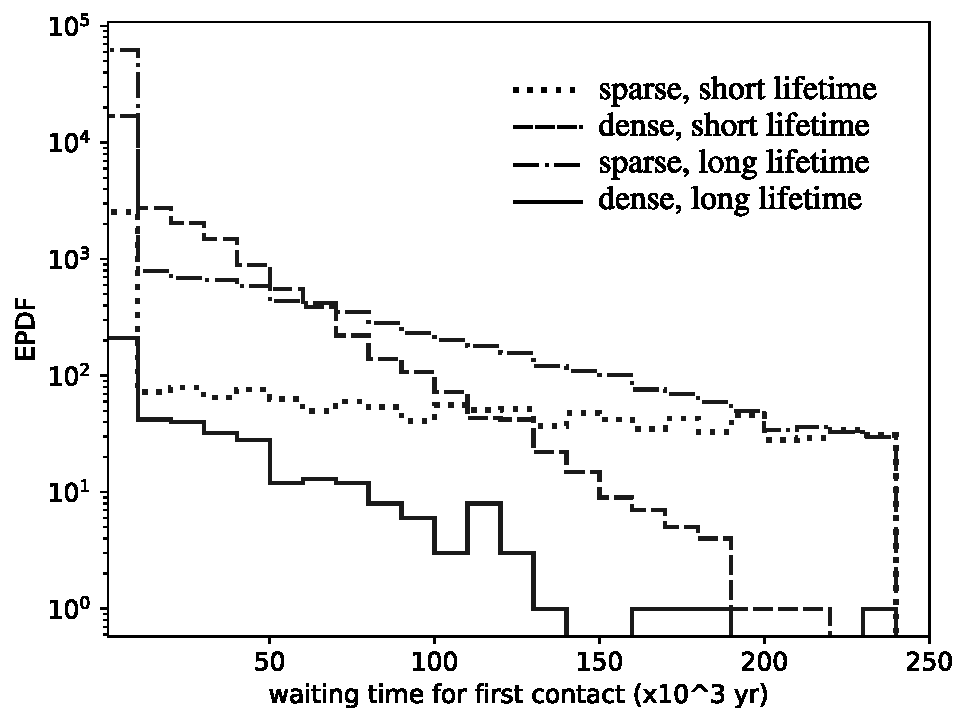
\includegraphics[width=0.5\textwidth]{F2.pdf}
   \caption{Rate of CETIs that make no contact as a function of
   $\tau_a$ and $\tau_s$}
   \label{F_res_2}
\end{figure}
 





 
\begin{figure*} % 2D color plot
   \centering
   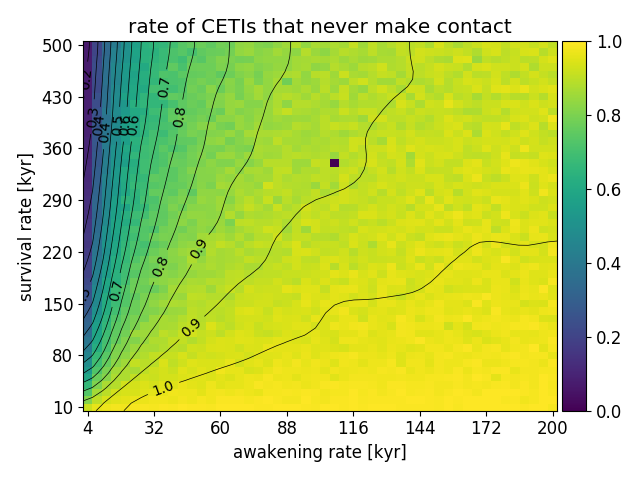
\includegraphics[width=0.3\textwidth]{m1d2.png}%
   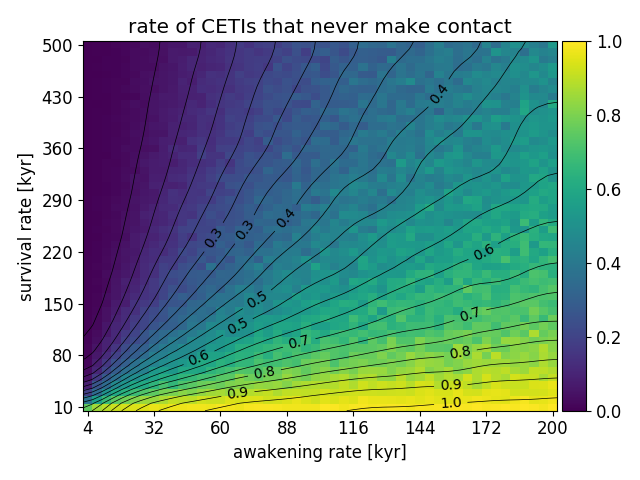
\includegraphics[width=0.3\textwidth]{m1d3.png}%
   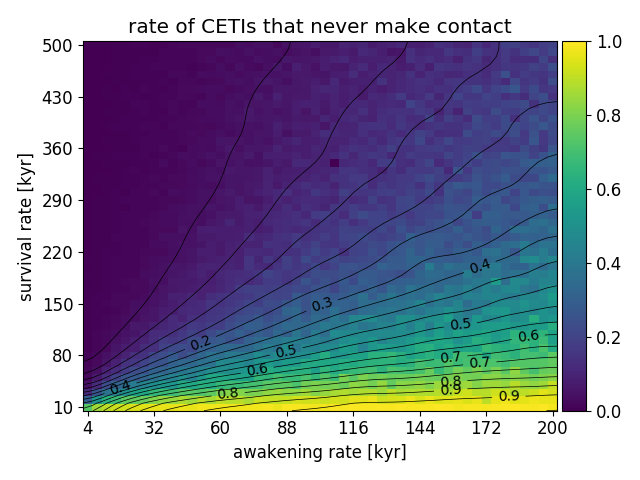
\includegraphics[width=0.3\textwidth]{m1d4.png}
   \caption{Rate of CETIs that never make contact (listening) as a
   function of $\tau_a$ and $\tau_s$, for 
   $D_{max}$=10000 (left panel),
   $D_{max}$=40000 (middle panel), and
   $D_{max}$=80000 (right panel)}
   \label{F_res_3}
\end{figure*}

  
\begin{figure*} % 2D color plot
   \centering
   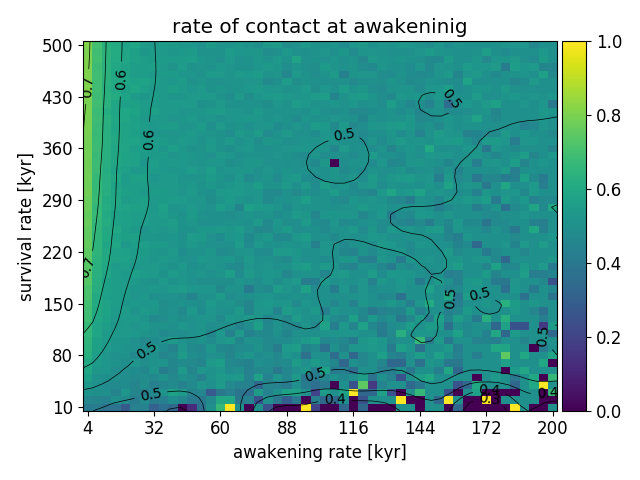
\includegraphics[width=0.3\textwidth]{m2d2.png}%
   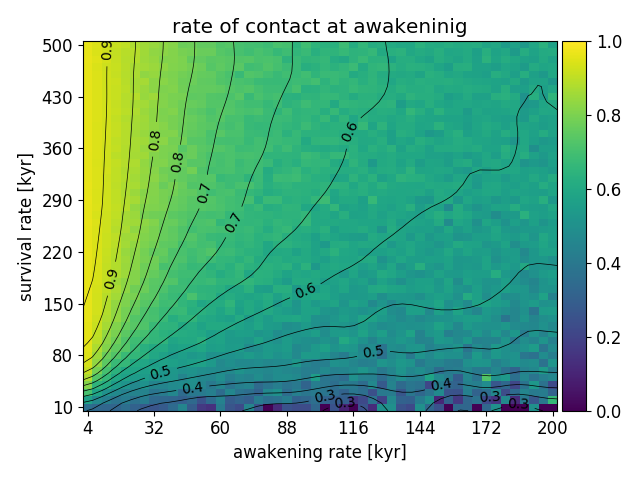
\includegraphics[width=0.3\textwidth]{m2d3.png}%
   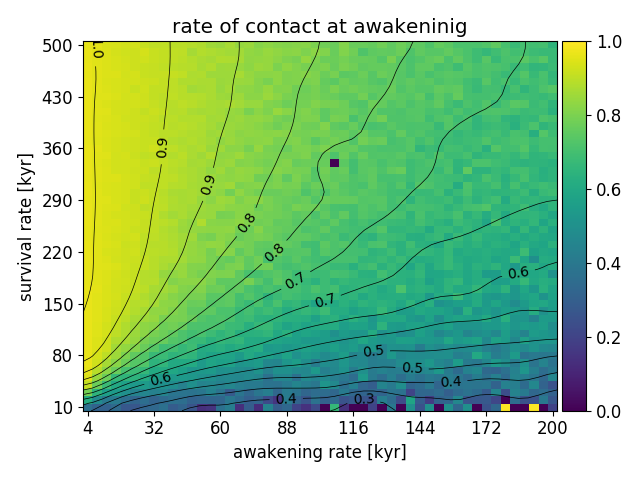
\includegraphics[width=0.3\textwidth]{m2d4.png}
   \caption{Rate of CETIs that listen at the moment of the
   awakening, as a funcion of $\tau_a$ and $\tau_s$}
   \label{F_res_4}
\end{figure*}



\begin{figure}
   \centering
   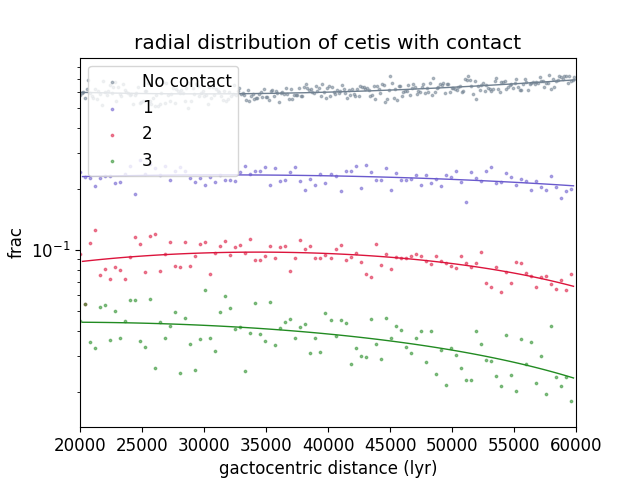
\includegraphics[width=0.5\textwidth]{radial.png}
   \caption{Fraction of CETIs making cero, one, two or three contacts as a function of
   galactocentric distance.}
   \label{F_res_5}
\end{figure}
           
 

\section{Discusion}\label{S_discussion}
%{{{

We have implemented a simulation approach to explore the hypothesis
space about the causal connections between communicating
extraterrestrial civilizations.
%
The different models can be generated with a minimal number of free
parameters and some fixed assumptions.
%
We argue that three parameters can be used to describe a variety of
situations, ranging from a Galaxy where an intelligent civilization is
very rare, to a Galaxy populated with plenty of civilizations in
causal contact.
%
We explored the consecuences of different models using mensurable
quantities.
%
With this approach, we can estimate several quantities as a function
of the parameters on the hypothesis space.
%
For instance, it is possible to estimate the timescale for an
uninterrupted SETI effort to reach success, in terms of different
model parameters that reflect different, so far unknown, scenarios
for the spread if intelligent life on the Galaxy.


Under the hypotheses of our experiments, we conclude that
a causal contact is extremely unlikely unless the Galaxy is heavily
populated by intelligent civilizations.
%
Even so, we must consider that in order to stablish a contact between
any two entities, a minimum degree of compatibility must be
accomplished without any previous agreement, 
making the posibility of a contact with a message that
could be deciphered highly rare.


Future work can be performed following this framework, in order to
explore possible implications of the results for more detailed 
configurations of the experiment.
%
For example, the communication method (isotropic, colimated,
serendipitous) can affect the observables.
%
Also the nature of the message carrier, electromagnetic or another.
%
It is also possible to explore the effects of alignments or the use of
stars as sources or amplifiers.
%
%energetic markers
%Spiritual markers
%
As a future work, we will explore several improvements to the
simulation, and analyze the impact on the final results of these
changes.
%
They include a spatial distribution that actually resembles the shape
of the Galaxy, different distribution functions for the mean lifetime
of CETIs and different efficiencies for the sphere of the causal
region of each CETI, resembling different searching strategies.
 
%}}}



\begin{figure*}
   \centering
   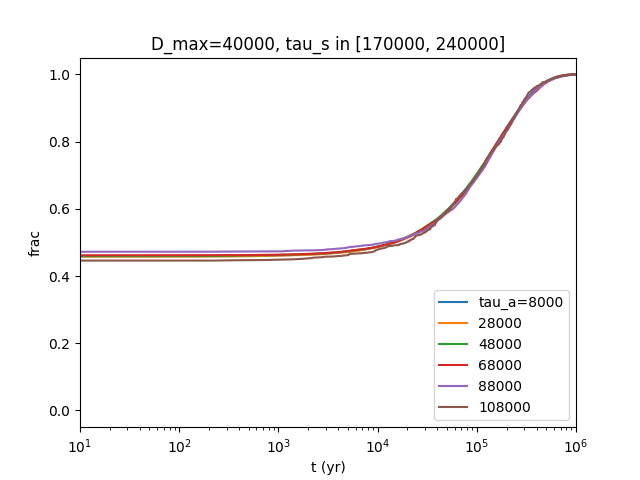
\includegraphics[width=0.33\textwidth]{waiting_a_acum_log.png}%
   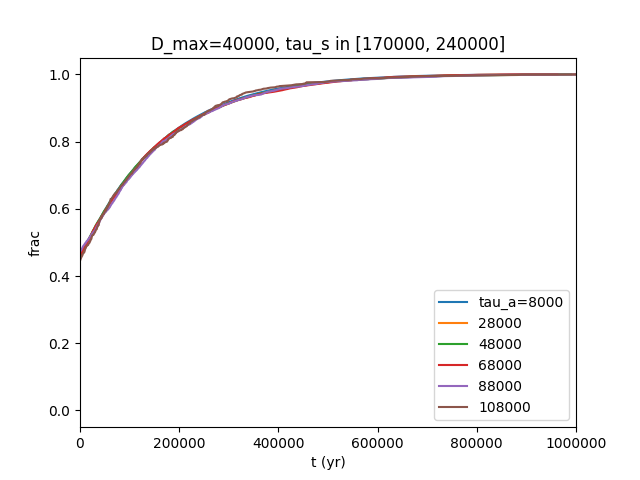
\includegraphics[width=0.33\textwidth]{waiting_a_acum_lin.png}%
   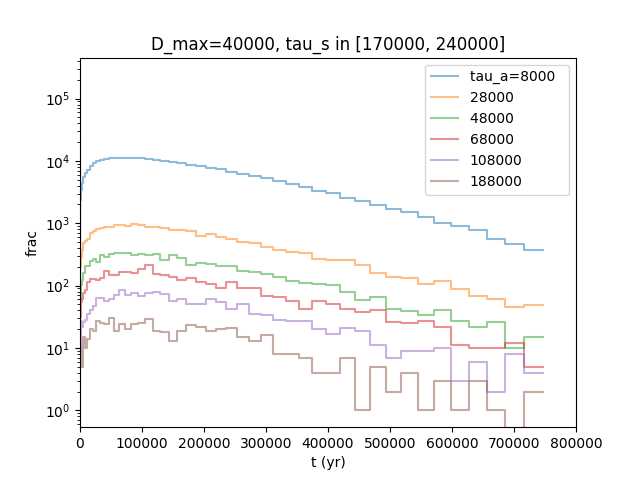
\includegraphics[width=0.33\textwidth]{waiting_a_dif.png}

   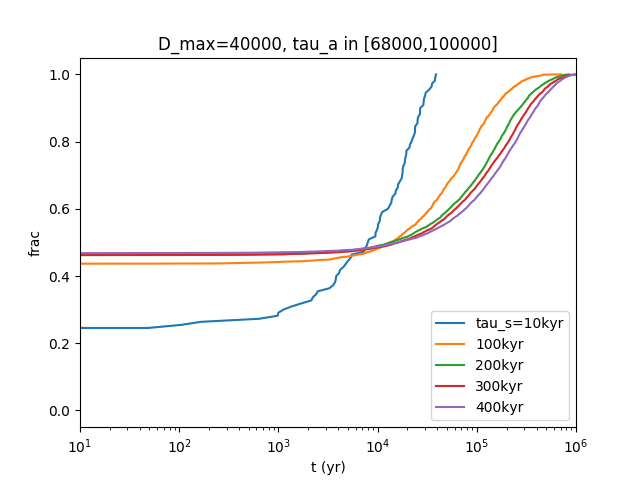
\includegraphics[width=0.33\textwidth]{waiting_s_acum_log.png}%
   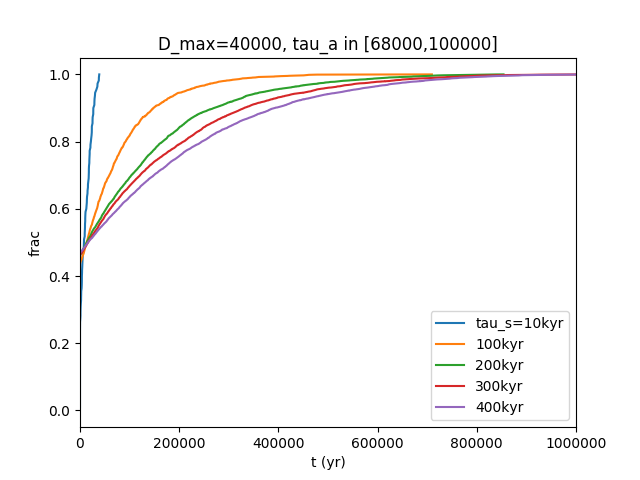
\includegraphics[width=0.33\textwidth]{waiting_s_acum_lin.png}%
   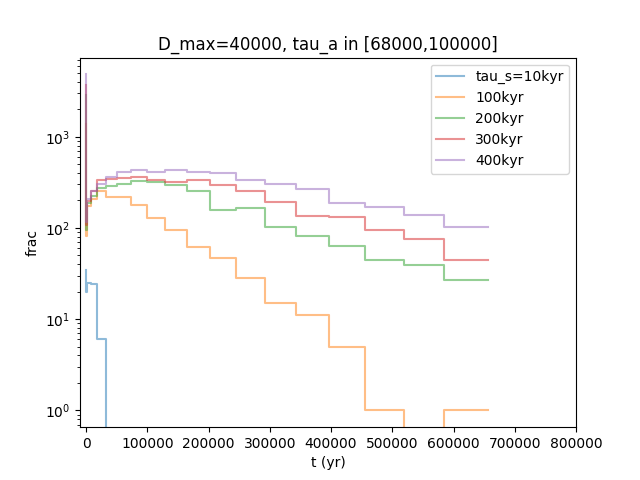
\includegraphics[width=0.33\textwidth]{waiting_s_dif.png}

   \caption{Fraction of the CETIs that have made at least one contact  
   as a funtion of the elapsed time since the awakening, given that
   they make at least one contact on their lifetime.
   %
   From a frequentist approach, this fraction is the estimation of the
   probability 
   
   }
   \label{F_waiting}
\end{figure*}

             


\begin{figure*}
   \centering
   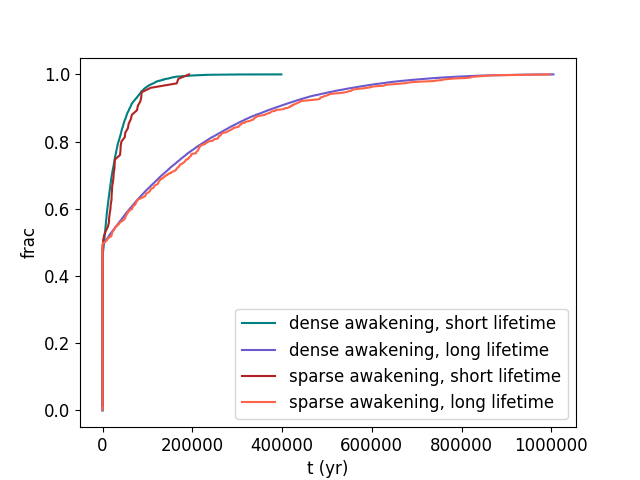
\includegraphics[width=0.33\textwidth]{prob1_10k.png}%
   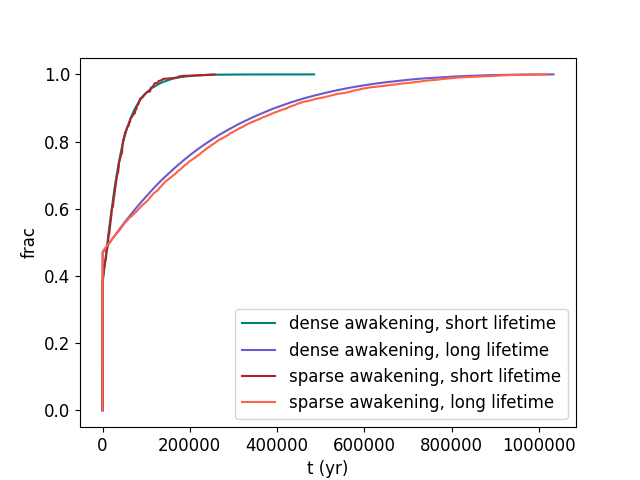
\includegraphics[width=0.33\textwidth]{prob1_40k.png}%
   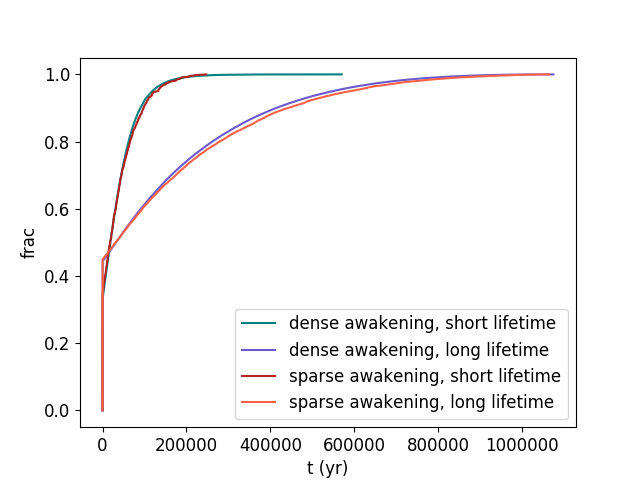
\includegraphics[width=0.33\textwidth]{prob1_80k.png}

   \caption{F_}
   \label{F_waiting}
\end{figure*}




                       


\ack[Acknowledgement]{
%
This work was partially supported by the Consejo Nacional de
Investigaciones Cient\'{\i}ficas y T\'ecnicas (CONICET, Argentina),
the Secretar\'{\i}a de Ciencia y Tecnolog\'{\i}a, Universidad Nacional
de C\'ordoba, Argentina, and the Universidad Católica de Córdoba,
Argentina.
%
This research has made use of NASA's Astrophysics Data System.
%
Plots and simulations were made with software developed by the authors
using R and python languajes, plots were postprocessed with inkscape.
%
}


\bibliography{biblio_seti}



\end{document}

DEVELOPMENT DEVELOPMENT  DEVELOPMENT  DEVELOPMENT  DEVELOPMENT  DEVELOPMENT  

% Papers para citar y discutir:

%## GHZ


%## D_max


%## exponential distribution


%## Lifetime


%## Simulations: cosmological

Forgan2015

%## Simulations: stochastic

grimaldi_signal_2017


%## Temporal aspects
Temporal aspects of the interaction among the first galactic civilizations: The 'interdict hypothesis'
by M.J. Fogg


%## Drake equation


%## Detalles de la simulacion
Galactic civilizations: Population dynamics and interstellar diffusion
by W.I. Newman, C. Sagan


